%!TEX root = slides.tex

\title{Data Representation and Querying}
\subtitle{}
\author{ian.mcloughlin@gmit.ie}
\date{}


\begin{frame}
	\titlepage
\end{frame}

\begin{frame}
	\frametitle{Topics}
	\tableofcontents
\end{frame}

\section{About this module}


\begin{frame}{Learning outcomes}
	On completion of this module the learner will/should be able to:
	\begin{itemize}
		\item Explain the benefits and the limitations of a variety of data models.
		\item Determine the most appropriate data model given a set of requirements.
		\item Represent, integrate and query large datasets using existing API's and frameworks.
		\item Describe the principles behind both the linked data and the open data movements.
	\end{itemize}
\end{frame}


\begin{frame}{Examinations}
	\begin{table}
		\begin{tabular}{p{4cm}r@{\hspace{0.5cm}}p{4cm}}
			Type & \% & Date \\
			\hline
			Project & 50 & Week 8 \\
			End of Semester Exam & 50 & See exams timetable
		\end{tabular}
	\end{table}
\end{frame}


\section{HTTP}

\begin{frame}{HyperText Transfer Protocol}
  \begin{description}
		\item[HyperText] Text with links.
    \vspace{0.25cm}
		\item[Transfer] Communication of data.
    \vspace{0.25cm}
		\item[Protocol] Set of rules for communication.
  \end{description}
\end{frame}


\begin{frame}{Request--Response}  
  \begin{adjustbox}{max width={0.9\textwidth},center} 
    \begin{tikzpicture}[node distance = 4cm]
      \node [oval] (client1) {Client (Firefox)};
      \node [rect, right of=client1] (request) {Request};
      \node [rect, right of=client1] (request) {Request};
      \node [oval, right of=request] (server1) {Server (Apache)};
      \node [rect, below=1cm of server1] (generate) {Generate response};
      \node [oval, below=1cm of generate] (server2) {Server (Apache)};
      \node [rect, left of=server2] (response) {Response};
      \node [oval, left of=response] (client2) {Client (Firefox)};
      \path [line] (client1) -- (request);
      \path [line] (request) -- (server1);
      \path [line,dashed] (server1) -- (generate);
      \path [line,dashed] (generate) -- (server2);
      \path [line] (server2) -- (response);
      \path [line] (response) -- (client2);
    \end{tikzpicture}
  \end{adjustbox}
\end{frame}


\begin{frame}{Uniform Resource Locator}
  \textcolor{amethyst}{http}://\textcolor{darkblue}{username}:\textcolor{davy\'sgrey}{password}@\textcolor{vermilion}{www}.\textcolor{azure(colorwheel)}{reddit.com}:\textcolor{brightpink}{80}\textcolor{green(ryb)}{/r/funny/}?\textcolor{harvardcrimson}{limit=1}
  
  \begin{table}
    \begin{tabular}{r@{\hspace{0.5cm}}p{6cm}}
      \textcolor{amethyst}{http} & Protocol \\
      \textcolor{darkblue}{username} & Username \\
      \textcolor{davy\'sgrey}{password} & Password \\
      \textcolor{vermilion}{www} & Subdomain \\
      \textcolor{azure(colorwheel)}{reddit.com} & Domain \\
      \textcolor{brightpink}{80} & Port \\
      \textcolor{green(ryb)}{/r/funny/} & Path \\
      \textcolor{harvardcrimson}{limit=1} & Parameter
    \end{tabular}
  \end{table}
\end{frame}


\begin{frame}{Resources}
 \begin{columns}[onlytextwidth]
   \begin{column}{0.5\textwidth}
     \centering
      \begin{figure}
        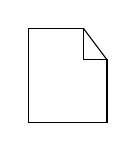
\begin{tikzpicture}
          \draw (0,0) -- (0,1.2) -- (0.7,1.2) -- (0.7,0.8) -- (1,0.8) -- (1,0) -- cycle;
          \draw (0.7,1.2) -- (1,0.8);
        \end{tikzpicture}
        \caption*{File}
      \end{figure}
    \end{column}
    \begin{column}{0.5\textwidth}
      \centering
      \begin{figure}
      \begin{tikzpicture}
        \node (A) [cylinder, shape border rotate=90, draw,minimum height=1.3cm,minimum width=1cm] {};
      \end{tikzpicture}
      \caption*{Database}
      \end{figure}
    \end{column}
  \end{columns}
  
  \begin{quote}
    HTTP is used to transmit resources \ldots A resource is some chunk of information that can be identified by a URL \ldots The most common kind of resource is a file, but a resource may also be a dynamically-generated query result \ldots
  \end{quote}
  \citeurl{www.jmarshall.com/easy/http}
\end{frame}


\begin{frame}{HTTP Methods}
  \begin{description}
    \item[GET] Retrieve information from the server.
    \item[HEAD] Like get, but retrieve only the response header.
    \item[POST] Send data to the server.
    \item[PUT] Set the resource at the URL to the request data.
    \item[DELETE] Delete the resource at the URL.
    \item[CONNECT] Set up tunnel for other traffic to pass through HTTP.
    \item[OPTIONS] Find the allowable operations at the given URL.
    \item[TRACE] Echo the received request.
    \item[PATCH] Partial resource modification.
  \end{description}
\end{frame}

\begin{frame}[fragile]{Request and Response Format}
  Requests and responses both have this format:
  \begin{itemize}
    \item Intial line.
    \item Zero or more header lines.
    \item A blank line.
    \item Optional message body (e.g. a HTML file)
  \end{itemize}
  \citeurl{www.jmarshall.com/easy/http}
\end{frame}


\begin{frame}[fragile]{Request (GET) Example}
  \begin{minted}{http}
GET /path/item/1?q=Funny+cats HTTP/1.0
From: someuser@jmarshall.com
User-Agent: HTTPTool/1.0
  \end{minted}
\end{frame}

\begin{frame}[fragile]{Request (POST)}
  \begin{minted}{http}
POST /path/script.cgi HTTP/1.0
From: frog@jmarshall.com
User-Agent: HTTPTool/1.0
Content-Type: application/x-www-form-urlencoded
Content-Length: 32

home=Cosby&favorite+flavor=flies
  \end{minted}
\end{frame}

\begin{frame}[fragile]{Response Example}
  \begin{minted}{http}
HTTP/1.1 200 OK
Date: Mon, 27 Jul 2009 12:28:53 GMT
Server: Apache/2.2.14 (Win32)
Last-Modified: Wed, 22 Jul 2009 19:15:56 GMT
Content-Length: 88
Content-Type: text/html
Connection: Closed

<html>
  <body>
    <h1>Hello, World!</h1>
  </body>
</html>
  \end{minted}
\end{frame}


\begin{frame}{URL encoding}
  HTML form data is usually URL-encoded by changing;
  \begin{itemize}
    \item Unsafe characters to \% \emph{xx} where \emph{xx} is the ASCII value.
    \item All spaces to plusses.
    \item Names and values to: name1=value1\&name2=value2.
  \end{itemize}
  
  \begin{description}
    \item[GET] Parameters go in the URL after ?, e.g.\ http://www.google.ie?q=Funny+cats.
    \item[POST] Parameters go in the body.
  \end{description}
  \citeurl{www.jmarshall.com/easy/http}
\end{frame}

\begin{frame}{Security}
  \begin{itemize}
    \item HTTP is not encrypted.
    \item HTTPS is a protocol based on HTTP, but it provides security.
    \item GET and POST are by far the most commonly used HTTP methods (by web developers).
    \item Data sent by GET and POST will be encrypted over HTTPS.
    \item However, it's generally accepted that POST is more secure for sending sensitive data.
    \item This is because browsers will typically cache and servers will typically log URLS, with the data encoded in them.
  \end{itemize}
\end{frame}


\section{REST}

\begin{frame}{REST}
  \begin{itemize}
    \item REST stands for Representational State Transfer.
    \item REST is an architecture describing how we might use HTTP.
    \item RESTful APIs make use of more HTTP methods than just GET and POST.
    \item Most HTTP APIs are not RESTful.
    \item RESTful APIs adhere to a few loosely defined constraints.
    \item Two of those constraints are that the API is stateless and cacheable.
  \end{itemize}
  \citeurl{drdobbs.com/web-development/restful-web-services-a-tutorial/240169069}
\end{frame}

\begin{frame}{Typical example}
  Suppose we have a system for storing and retrieving emails.
  \begin{table}
    \begin{tabular}{r@{\hspace{0.5cm}}|l@{\hspace{0.5cm}}|l}
      Method & URL & Description \\
      \hline
      GET    & /emails   & list all emails \\
      POST   & /email    & store new email \\
      GET    & /email/32 & retrieve email with id 32 \\
      PUT    & /email/32 & update email with id 32 \\
      DELETE & /email/32 & delete email with id 32
    \end{tabular}
  \end{table}
  \citeurl{bitworking.org/news/201/restify-daytrader}
\end{frame}

\begin{frame}{Stateless}
  \begin{itemize}
    \item Statelessness is a REST constraint.
    \item HTTP uses the client-server model.
    \item The server should treat each request as a single, independent transaction.
    \item No client state should be stored on the server.
    \item Each request must contain all of the information to perform the request. 
  \end{itemize}
\end{frame}

\begin{frame}{Cacheable}
  \begin{itemize}
    \item REST APIs should provide responses that are cacheable.
    \item Intermediaries between the client and server should be able to cache responses.
    \item This should be transparent to the client.
    \item Cacheability increases response time.
    \item Browsers usually cache resources, in case they are requested again.
    \item There is usually a time limit on cached resources.
  \end{itemize}
\end{frame}



\section{JSON}

\begin{frame}{JSON}
  \begin{description}
    \item[JavaScript] A scripting/programming language.
    \vspace{0.25cm}
    \item[Object] Groups of name--value pairs.
    \vspace{0.25cm}
    \item[Notation] Set of rules for representing objects.
  \end{description}
\end{frame}

\begin{frame}{About JSON}
  \begin{itemize}
    \item JSON is just text, but text that conforms to a syntax.
    \item JSON is heavily influenced by JavaScript, but it is used in with all languages.
    \item JSON's primary purpose is to represent information in text form.
    \item JSON is popular because it is easy to send over HTTP and parse in JavaScript.
  \end{itemize}
\end{frame}

\begin{frame}{Sending JSON}
  \tikzstyle{block} = [rectangle, fill=azure(colorwheel), text width=4.5em, text centered, minimum height=4em]
  \tikzstyle{line} = [draw, -latex']
  \tikzstyle{cloud} = [ellipse, fill=wildwatermelon, text width=5em, text centered]
  \tikzstyle{startstop} = [rectangle, rounded corners, text width=5em, minimum height=4em, text centered, fill=tiffanyblue]
  
  \begin{adjustbox}{max totalsize={.9\textwidth}{.6\textheight},center} 
    \begin{tikzpicture}[node distance=4cm]
    \node [oval] (object1) {Object Instance};
    \node [rect, below of=object1] (json1) {JSON};
    \node [rect, right of=json1, node distance = 6cm] (json2) {JSON};
    \node [oval, above of=json2] (object2) {Object Instance};
    % Draw edges
    \path [line] (object1) -- node[style={rectangle,fill=white,draw}]{stringify} (json1);
    \path [line] (json1) -- node[style={rectangle,fill=white},draw ]{HTTP} (json2);
    \path [line] (json2) -- node[style={rectangle,fill=white,draw}]{parse} (object2);
    % Draw Memory
    \draw [color=gray, dashed](-2,-1.5) rectangle (2,1.25);
    \node at (-1.4,-1.35) [] {\tiny Machine 1};
    \draw [color=gray, dashed](4,-1.5) rectangle (8,1.25);
    \node at (4.6,-1.35) [] {\tiny Machine 2};
    \end{tikzpicture}
  \end{adjustbox}
\end{frame}

\begin{frame}[fragile]{JSON Example}
  \begin{minted}{json}
{
  "employees": [
    {"firstName":"John", "lastName":"Doe"},
    {"firstName":"Anna", "lastName":"Smith"},
    {"firstName":"Peter", "lastName":"Jones"}
  ]
}
  \end{minted}
\end{frame}

\begin{frame}[fragile]{Using JSON in JavaScript}
  \begin{minted}{javascript}
// Turning text into a JavaScript object.
var obj = JSON.parse(text);
// obj is an obect.

// Turning a JavaScript object into text.
var text = JSON.stringify(obj);
// text is a string.
  \end{minted}
\end{frame}

\begin{frame}{JSON Syntax}
  \begin{itemize}
    \item Name/Value pairs separated by a colon. \\
    \hspace{0.5cm} \mintinline{json}{"name": "Ian"}
    \item Objects identified by curly braces. \\
    \hspace{0.5cm} \mintinline{json}{{}}
    \item Lists identified by square brackets. \\
    \hspace{0.5cm} \mintinline{json}{[]}
    \item All strings (and names) use double quotes (not single). \\
    \hspace{0.5cm} \mintinline{json}{"Ian"}
  \end{itemize}
\end{frame}

\begin{frame}{JSON Types}
  \begin{itemize}
    \item Numbers \\
    \hspace{0.5cm} \mintinline{json}{123.456}
    \item Strings \\
    \hspace{0.5cm} \mintinline{json}{"Hello, world!"}
    \item Boolean \\
    \hspace{0.5cm} \mintinline{json}{true"}
    \item Arrays\\
    \hspace{0.5cm} \mintinline{json}{[1,2,3]}
    \item Objects\\
    \hspace{0.5cm} \mintinline{json}{{"name": "Ian"}}
    \item null \\
    \hspace{0.5cm} \mintinline{json}{null}
  \end{itemize}
\end{frame}

\section{XML}

\begin{frame}{eXtensible Markup Language}
  \begin{description}
    \item[Extensible] Designed to accommodate change.
    \vspace{0.25cm}
    \item[Markup] Annotates text.
    \vspace{0.25cm}
    \item[Language] Set of rules for communication.
  \end{description}
\end{frame}


\begin{frame}{About XML}
  \begin{itemize}
    \item XML is an alternative to JSON.
    \item XML looks like HTML, but it is different.
    \item XML's purpose is to represent information in text form.
    \item There are no pre-defined tag names -- you make them up yourself.
    \item XML has a tree-like syntax.
    \item The Document Object Model (DOM) can be applied to XML.
  \end{itemize}
\end{frame}

\begin{frame}[fragile]{XML Example}
  \begin{minted}{xml}
<?xml version="1.0" encoding="UTF-8"?>
<book isbn-13="978-0131774292" isbn-10="0131774298">
  <title>Expert C Programming: Deep C Secrets</title>
  <publisher>Prentice Hall</publisher>
  <author>Peter van der Linden</author>
</book>
  \end{minted}
\end{frame}

\begin{frame}{XML Syntax}
  \begin{description}
    \item[Declaration] XML documents should have a single line at the start stating that it's XML, the version of XML it is, and an encoding.
    \item[Elements] XML is structured as elements, which are enclosed in angle brackets.
    \item[Root element] XML must have a single root element that wraps all others.
    \item[Attbirutes] Elements can have attributes, which are name--value pairs within the angle brackets. A given attribute name can only be specified once per element.
    \item[Entity references] Certain characters must be escaped with entity references, e.g.\ \&lt; for $\langle$.
    \item[Case sensitive] Everything in XML is case sensitive.
  \end{description}
\end{frame}

\begin{frame}[fragile]{XML Syntax Example}
  \begin{minted}{xml}
  <?xml version="1.0" encoding="UTF-8"?>
  <parent-element attribute-name="attribute-value">
    <child name="value">Text</child-element>
    <child name="value">Text</child-element>
    <child name="value">Text</child-element>
    <lone-warrior />
  </parent-element>
  \end{minted}
\end{frame}

\begin{frame}{Document Object Model}
  \begin{itemize}
    \item The Document Object Model (DOM) is a programming interface for HTML and XML documents.
    \item It provides a model of the document as a structured group of nodes that have properties and methods.
    \item The DOM connects web pages to scripts or programming languages.
    \item You can use document.createElement, document.createTextNode and document.element.appendChild to add to the DOM.
    \item You can use document.getElementById to access elements of the DOM.
  \end{itemize}
  \citeurl{developer.mozilla.org/en-US/docs/Web/API/Document\_Object\_Model/Introduction}
\end{frame}


\section{AJAX}

\begin{frame}{Asynchronous JavaScript and XML}
  AJAX stands for Asynchronous JavaScript and XML.
  \vspace{0.5cm}
  \begin{description}
    \item[Asynchronous] In the background, and without a page refresh.
    \vspace{0.25cm}
    \item[JavaScript] Programming language for the web.
    \vspace{0.25cm}
    \item[XML] eXtensible Markup Language.
  \end{description}
\end{frame}


\begin{frame}{About AJAX}
  \begin{itemize}
    \item AJAX allows us to make a HTTP request from JavaScript without a page refresh.
    \item AJAX also allows us to receive the response from that request and deal with it.
    \item Despite the name, we don't have to use XML -- we can use JSON or anything else.
    \item This happens asynchronously, so that the rest of our code be run while waiting for a slower piece of code to complete.
    \item HTTP requests are usually relatively slow.
    \item We use a callback function, which is called when the HTTP transaction is complete.
  \end{itemize}
\end{frame}

\begin{frame}[fragile]{AJAX Example}
  \begin{minted}{javascript}
var xmlhttp = new XMLHttpRequest();

xmlhttp.onreadystatechange = function() {
  if (xmlhttp.readyState == 4) {
    var mydiv = document.getElementById("mydivid");
    mydiv.innerHTML = xmlhttp.responseText;
  }
};

xmlhttp.open("GET", "https://goo.gl/2GCplC");
xmlhttp.send();
  \end{minted}
\end{frame}

\begin{frame}{AJAX Example Explained}
  \begin{itemize}
    \item XMLHttpRequest is a built-in class that provides AJAX functionality in JavaScript.
    \item httpRequest.onreadystatechange should be set to a function to run every time something happens in our HTTP call.
    \item httpRequest.open is called to initialize the request.
    \item httpRequest.send is used to send the request to the server.
    \item XMLHttpRequest.readyState changes when the state of the AJAX call changes. This triggers a call to httpRequest.onreadystatechange.
  \end{itemize}
\end{frame}

\begin{frame}[fragile]{Using jQuery}
  \begin{minted}{html}
<script src="jquery.min.js"></script>
  \end{minted}
  \vspace{1cm}
  \begin{minted}{javascript}
$.get("https://goo.gl/2GCplC", function(data) {
  $("#mydivid").html(data);
});
  \end{minted}
\end{frame}


\section{HTTP APIs}


\begin{frame}{HTTP APIs}
	\begin{itemize}
		\item Facebook, Google, Reddit and others often provide programmable interfaces to their services.
		\item This lets other application developers use the services programmatically.
		\item For instance, Reddit allows developers to create mobile apps for viewing and making submissions to reddit.
		\item HTTP is often the mechanism used for this purpose.
		\item Access is provided through a set of URLs, across a variety of HTTP methods.
		\item The APIs often require JSON in HTTP request bodies and often return the query results as JSON.
	\end{itemize}
\end{frame}



\section{NoSQL}

\begin{frame}{NoSQL}
	\begin{itemize}
		\item NoSQL is the umbrella term for databases that do not conform to the relational, SQL-style model.
		\item Relational databases are good for some types of data.
		\item However, they have some issues.
		\item SQL queries can result in costly joins.
		\item Tables can be sparsely populated.
		\item Two common NoSQL database types are Document-oriented and Graph.
		
	\end{itemize}
\end{frame}

\begin{frame}{CouchDB}
	\begin{itemize}
		\item CouchDB is a document-oriented database.
		\item Documents are represented in CouchDB as JSON objects.
		\item Each document has its own id and revision, indicated by properties \mintinline{js}{_id} and \mintinline{js}{_rev} in the JSON document.
		\item Updating a document leaves its \mintinline{js}{_id} intact, but updates its \mintinline{js}{_rev}.
		\item Different documents can have different properties -- there is no schema.
		\item The main interface with CouchDB, for storage and retrieval is a HTTP API.
		\item CouchDB uses HTTP methods such as \mintinline{http}{GET}, \mintinline{http}{POST}, \mintinline{http}{PUT} and \mintinline{http}{DELETE} to retrieve, add, update and delete documents.
	\end{itemize}
\end{frame}

\begin{frame}{Futon}
	\begin{itemize}
		\item CouchDB has an in-built admin interface.
		\item It's called Futon.
		\item You access it through the \mintinline{html}{/_utils} path.
		\item You can create and delete databases.
		\item You can also create, update and delete documents.
	\end{itemize}
\end{frame}


\section{MapReduce}

\begin{frame}{MapReduce}
	\begin{itemize}
		\item MapReduce is a way of programming.
		\item It is a model performing specific types of problems that are common in programming.
		\item MapReduce promotes algorithms that have an initially embarrassingly parallel part, and a subsequent consolidation part.
		\item The former is the Map part, and the letter is the Reduce part.
		\item MapReduce isn't necessarily anything new, the ideas have existed for a long time.
		\item The formalisation of those ideas and their implementation in systems such as Hadoop is useful.
	\end{itemize}
\citeurl{joelonsoftware.com/items/2006/08/01.html}
\end{frame}

\begin{frame}[fragile]{Map}
Map takes a function and a list, and applies the function to every element of the list.
  \begin{minted}{javascript}
function map(fn, a) {
  r = [];
  for (i = 0; i < a.length; i++)
  	r[i] = fn(a[i]);
	return r;
}
	\end{minted}
	\citeurl{joelonsoftware.com/items/2006/08/01.html}
\end{frame}

\begin{frame}[fragile]{Reduce}
Reduce takes the output of Map, and accumulates the elements in some way.
  \begin{minted}{javascript}
function reduce(fn, a, init) {
  var s = init;
  for (i = 0; i < a.length; i++)
      s = fn(s, a[i]);
  return s;
}
	\end{minted}
	\citeurl{joelonsoftware.com/items/2006/08/01.html}
\end{frame}

\begin{frame}[fragile]{Map Reduce in CouchDB}
Reduce takes the output of Map, and accumulates the elements in some way.
  \begin{minted}{javascript}
function(doc) {
  if(doc.date && doc.title) {
    emit(doc.date, doc.title);
  }
}
	\end{minted}
	
  \begin{minted}{javascript}
function(keys, values, rereduce) {
  if (rereduce)
    return sum(values);
	else
    return values.length;
}
	\end{minted}
	
	\citeurl{http://guide.couchdb.org/draft/views.html}

\end{frame}